\documentclass[main]{subfiles}

\begin{document}

\chapter{Filtro de Kalman}

Se desea implementar algún algoritmo de estimación de estados que, corriendo en tiempo real, mantenga una estimación del estado mejor que la que se obtendría utilizando solamente las medidas de los sensores, agregando robustez a las medidas obtenidas, y logrando estimar variables de estado que no se miden directamente de los sensores.\\

El filtro de Kalman es un algoritmo que usa una serie de medidas ruidosas observadas a lo largo del tiempo y produce una estimación de alguna variable desconocida que resulta ser más precisa que la observación llana de la medidas. Opera recursivamente sobre el flujo de la entrada ruidosa y arroja la estimación estadísticamente óptima del estado.

Consiste básicamente en 2 etapas:
\begin{itemize}
  \item Predicción
  \item Actualización
\end{itemize}

En la figura \ref{fig:kal} se muestra un diagrama de flujo de la operación de un filtro de Kalman. Se parte de una estimación a priori del estado, la cual es utilizada como semilla para las posteriores iteraciones del filtro. En la etapa de \textbf{predicción}, el filtro produce una estimación del estado de las variables, junto con sus incertidumbres. Se hallan las variables $P_{k|k-1}$ y $\hat{x}_{k|k-1}$, correspondientes a la predicción de la matriz de covarianza estimada y la predicción del estado estimado, respectivamente. La covarianza, en la teoría de la probabilidad, es una medida de cuán juntas cambian 2 variables aleatorias. Si presentan un comportamiento similar tendrán una covarianza elevada y positiva, si el comportamiento es opuesto la covarianza será negativa y elevada en valor absoluto. Si las variables aleatorias no presentan relación, la covarianza será 0. Es una magnitud que no es sencilla de interpretar pero cobra vital importancia a la hora de entender el comportamiento del filtro y resulta ser la herramienta más clara para regular la influencia de la predicción y de la corrección, como se verá más adelante.\\

\begin{figure}[h!]
	\centering
	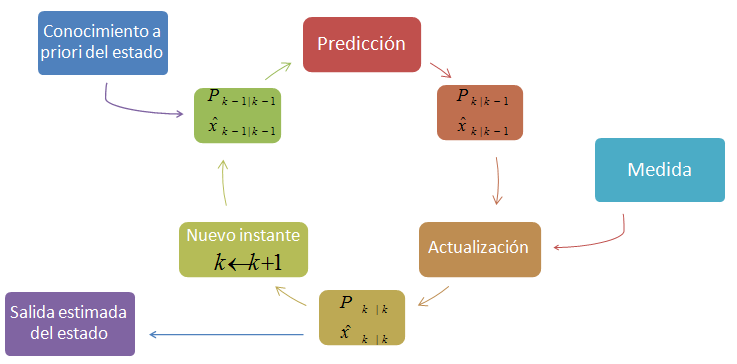
\includegraphics[width=.8\textwidth]{./pics_kalman/kal.png}
	\caption{Diagrama de flujo del filtro de Kalman}
	\label{fig:kal}
\end{figure}

Una vez que llega la siguiente medida de los sensores, necesariamente contaminada con ruido, las estimaciones son actualizadas en la etapa de \textbf{actualización}, mediante la utilización de un \emph{promedio ponderado}, dándole mayor peso a las estimaciones con menor incertidumbre en cada paso, obteniendo la estimación del estado para el instante k: $P_{k|k}$ y $\hat{x}_{k|k}$.\\

Por otro lado, las mayores restricciones que impone el filtro de Kalman son que el sistema dinámico subyacente debe ser lineal y que los ruidos presentes deben ser blancos y Gaussianos.\\

El sistema dinámico que queremos estimar, como se puede ver en el capítulo \ref{chap:modelo}, es claramente \textbf{no lineal}, por lo que se debe buscar alguna alternativa al filtro de Kalman clásico. Al investigar en la literatura existente, basados en \cite{bib:kalman} y \cite{bib:kalman2}, se decide implementar un filtro de \emph{Kalman extendido} para la estimación del vector de estados.

\section{Filtro de Kalman Extendido (EKF)}

El filtro de \emph{Kalman extendido (EKF)} es la versión no lineal del filtro de Kalman. Linealiza en torno a una estimación de la media y la covarianza. En caso de conocer con exactitud el modelo de transición de estados, el EKF se considera el estándar en la estimación no lineal aplicada a sistemas de navegación.\\

\subsection{Modelo matemático}

El sistema dinámico sigue el modelo:

$$\mathbf{x}_{k} = f(\mathbf{x}_{k-1}, \mathbf{u}_{k-1}) + \mathbf{w}_{k-1}$$

$$\mathbf{z}_{k} = h(\mathbf{x}_{k}) + \mathbf{v}_{k}$$

donde $\mathbf{w}_k$ y $\mathbf{v}_k$ son los ruidos de proceso y observación respectivamente. Se asume que son gaussianos y de media nula. Sus matrices de covarianza son $\mathbf{Q}_k$ y $\mathbf{R}_k$ respectivamente.

La función $f$ es utilizada para hallar el estado predicho a partir del estado previo, y de forma análoga la función $h$ se utiliza para hallar la medida predicha a partir del estado. Dicho de otro modo, la función $f$ guarda información sobre la evolución del estado, mientras que la función $h$ representa la transformación entre el vector de estados y la observación ideal (sin ruido). Dada la no linealidad del sistema, las funciones $f$ y $h$ no pueden ser aplicadas directamente a la covarianza. En su lugar se computa su \textbf{Jacobiano}, una matriz de derivadas parciales. Es importante destacar que el filtro de Kalman Extendido no tiene propiedades de optimalidad y su precisión dependerá en gran medida de la precisión de la linealización. Dado que se realiza una linealización dinámica, no hay manera de conocer su performance de antemano (por mayor detalles referirse a \cite{bib:kay}).\\
Para la predicción del estado se utilizan las ecuaciones del modelo físico del cuadricóptero presentadas en el capítulo \ref{chap:modelo}.\\

Las ecuaciones que gobiernan el comportamiento del filtro de Kalman Extendido son:
\begin{itemize}
	\item Predicción:
	\begin{itemize}
		\item Estimación de la predicción del estado
		$$\hat{\mathbf{x}}_{k|k-1} = f(\hat{\mathbf{x}}_{k-1|k-1}, u_{k-1})$$
		\item Estimación de la predicción de la covarianza
		$$ \mathbf{P}_{k|k-1} =  {{\mathbf{F}_{k-1}}} \mathbf{P}_{k-1|k-1}{  {\mathbf{F}_{k-1}^T}} + \mathbf{Q}_{k-1} $$		
	\end{itemize}
	\item Actualización
	\begin{itemize}
		\item Residuo de medida
		$$\tilde{\mathbf{y}}_{k} = \mathbf{z}_{k} - h(\hat{\mathbf{x}}_{k|k-1})$$
		\item Residuo de covarianza
		$$\mathbf{S}_{k} = { \mathbf{H}_{k}}\mathbf{P}_{k|k-1}{ \mathbf{H}_{k}^\top} + \mathbf{R}_{k}$$
		\item Ganancia de Kalman
		$$\mathbf{K}_{k} = \mathbf{P}_{k|k-1}{ \mathbf{H}_{k}^\top}\mathbf{S}_{k}^{-1} $$
		\item Estimación actualizada del estado
		$$\hat{\mathbf{x}}_{k|k} = \hat{\mathbf{x}}_{k|k-1} + \mathbf{K}_{k}\tilde{\mathbf{y}}_{k} $$
		\item Estimación actualizada de la covarianza.
		$$ \mathbf{P}_{k|k} = (I - \mathbf{K}_{k} { \mathbf{H}_{k}}) \mathbf{P}_{k|k-1} $$		
	\end{itemize}
\end{itemize}

Las matrices de transición de estados y observación son los siguientes jacobianos:
$$ { \mathbf{F}_{k-1}} = \left . \frac{\partial f}{\partial \mathbf{x} } \right \vert _{\hat{\mathbf{x}}_{k-1|k-1},\mathbf{u}_{k-1}} $$
\vspace{10pt}
$$ { \mathbf{H}_{k}} = \left . \frac{\partial h}{\partial \mathbf{x} } \right \vert _{\hat{\mathbf{x}}_{k|k-1}} $$


\subsection{Esquema general del estimador de estados}

Los datos (en algunos casos redundantes) obtenidos de los diferentes sensores son combinados usando un filtro de Kalman Extendido para determinar el vector de estados, detallado en \ref{chap:modelo}:
\begin{equation}
  \label{eq:estado}
  X=\left\lbrace  x,y,z,\psi,\varphi,\theta, v_{q_x},v_{q_y},v_{q_z},\omega_{q_x},\omega_{q_y},\omega_{q_z} \right\rbrace
\end{equation}

De la caracterización de los motores, capítulo \ref{chap:test_motores}, se obtienen las ecuaciones que rigen la fuerza y el torque de \emph{drag} de cada motor, funciones que dependen solamente de su velocidad de giro. Por lo tanto, basta con controlar la velocidad de giro de los motores para poder determinar todas las entradas al sistema. Se considerará entonces como entrada al sistema las velocidades angulares $w_1$, $w_2$, $w_3$, $w_4$ de los 4 motores.\\

El esquema general del integración de los sensores se puede ver en la figura \ref{fig:diagrama_kalman}, el cual se pasa a describir a continuación.

\begin{figure}[h!]
	\centering
	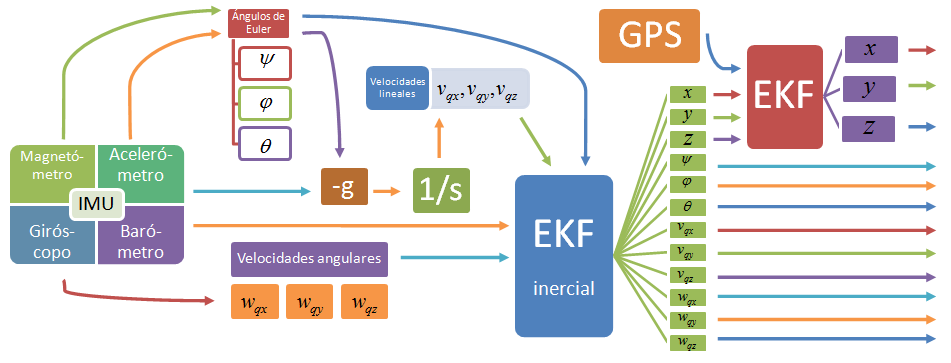
\includegraphics[width=1\textwidth]{./pics_kalman/diagrama_kalman.png}
	\caption{Esquema general de integración de sensores}
	\label{fig:diagrama_kalman}
\end{figure}

Básicamente se utilizan 2 filtros de Kalman distintos.\\
El primero (Kalman inercial) se encarga de estimar los 12 estados del vector $X$ considerando solamente las medidas obtenidas del sensor inercial (\textbf{IMU}): acelerómetros, giróscopos, magnetómetro, barómetro y termómetro. Para la estimación de los ángulos se utiliza una combinación entre las medidas obtenidas del acelerómetro y del magnetómetro, para la estimación de las velocidades angulares se utiliza directamente la medida arrojada por el giróscopo y para las velocidades lineales se trabaja con las medidas arrojadas por el acelerómetro. A su vez, al estar considerado el modelo físico dentro del filtro, se utilizan las estimaciones de todas las variables para determinar las predicciones del resto. Para la estimación de la posición en ``x'' y en ``y'' no se tiene ninguna medida de corrección, por lo que quedará determinado únicamente por la predicción del modelo físico, lo cual resulta en una acumulación significativa de error.
El segundo se encarga de la integración de los datos recogidos por el GPS, logrando una corrección en las posiciones y velocidades lineales gracias a la realimentación de la posición entregada por el GPS. En este caso se resuelve el problema de acumulación de error del filtro inercial.\\

La separación en 2 filtros distintos otorga una interesante flexibilidad. Es posible utilizar una estimación del estado estando a puertas cerradas, sin la necesidad de señal de GPS, a costas de una peor estimación de las posiciones y velocidades lineales en ``x'' e ``y''. Además la frecuencia de muestreo del GPS es mucho más baja que la del resto de los sensores, por lo cual se hace imprescindible la utilización de un filtro meramente inercial. Los datos de la IMU llegan cada $10ms$, mientras que los del GPS cada $1s$, entonces mientras no se tiene un dato nuevo de GPS, se utiliza la estimación inercial de las posiciones y cuando llega un dato nuevo de GPS es utilizado como corrección, dándole mucho más peso que a la estimación inercial, para evitar el $drift$ mencionado.

\subsubsection*{Orientación}

En estado estático, los ángulos de \emph{pitch} y \emph{roll} pueden ser determinados proyectando el vector medido de aceleración gravitacional por el acelerómetro. A su vez, los cambios entre el sensor magnético y el vector geomagnético medido, representan al ángulo \emph{yaw}. Por lo tanto, el conjunto del acelerómetro y magnetómetro son capaces de determinar la orientación del cuadricóptero mediante las medidas del vector de aceleración gravitatoria y el vector geomagnético. Dado que el magnetómetro digital no introduce acumulación de error, este sistema ha sido muy utilizado para la determinación estática de la posición, como se puede ver en \cite{bib:euler_magneto_acc}. Una observación no menor es que en el pasaje de estado estático al vuelo, lo antes dicho sobre los ángulos \emph{pitch} y \emph{roll} sigue siendo válido ya que las aceleraciones que puedan aparecer en vuelo resultan despreciables frente a la aceleración de la gravedad.

\subsubsection{Aceleración}

Para poder obtener la transformación entre el vector de estados y la observación es necesario entender qué aceleración medirá el acelerómetro. Como se explica en \ref{acelerometro}, dicho dispositivo referencia su medida a un sistema en caída libre, por lo que por ejemplo al estar quieto se deberá medir la aceleración gravitatoria ($g$).\\
Como se puede ver en el esquema mostrado en la figura \ref{fig:diagrama_kalman}, el acelerómetro es utilizado para estimar las variables de estado $v_{qx}$, $v_{qy}$ y $v_{qz}$, correspondientes a las velocidades lineales medidas en el sistema del cuadricóptero. No se debe confundir la derivada de estas variables con la aceleración medida por el acelerómetro. Por un lado se debe realizar el pasaje del sistema de referencia del cuadricóptero hasta un sistema de referencia inercial fijo en el mundo, y por otro lado se debe tener en cuenta el pasaje de este último hasta el sistema de referencia del acelerómetro (el sistema en caída libre), por ello es que se incluye el bloque ``-g'' en el diagrama de la figura \ref{fig:diagrama_kalman}.

% TODO hablar de Q y R. capaz poner 2 ejemplos de lo mismo q den bien distinto


\section{Resultados: Kalman inercial}

\subsection{Simulación de vuelo}
\subsubsection{Hovering}
La trayectoria de \emph{Hovering} consiste en que el cuadricóptero permanezca suspendido en el aire en el lugar. Para simular esta situación se setea como entrada una velocidad angular en los motores calculada para equilibrar la fuerza del peso de cuadricóptero.
Se presentan a continuación algunos resultados de la implementación del filtro de Kalman como estimador del vector de estados.\\

\begin{figure} [h!]
\centering
  \subfloat[Velocidad angular referenciada al cuadricóptero]{\label{fig:wq}
    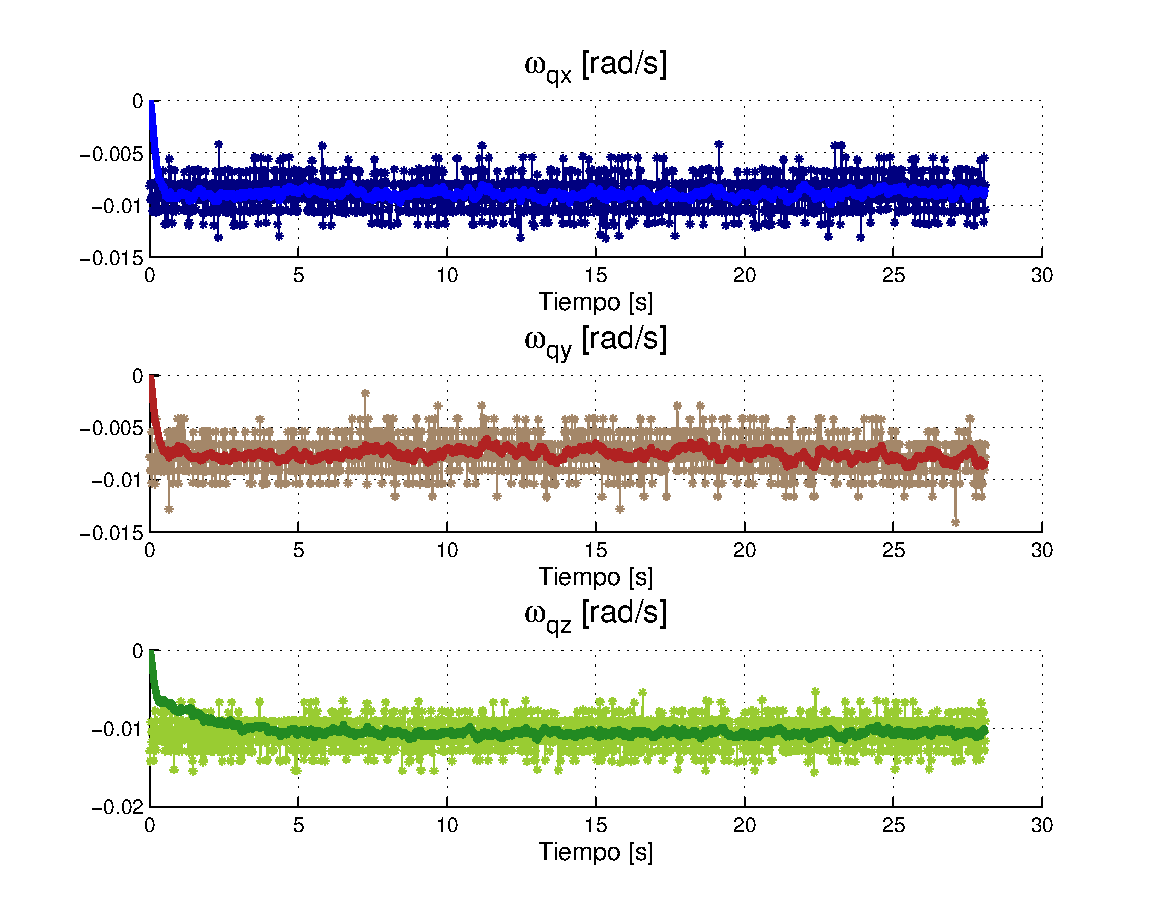
\includegraphics[width=0.47\textwidth]{./pics_kalman/wq.pdf}} \hspace{10pt}
  \subfloat[Orientación del cuadricóptero según ángulos de euler]{\label{fig:euler} 
    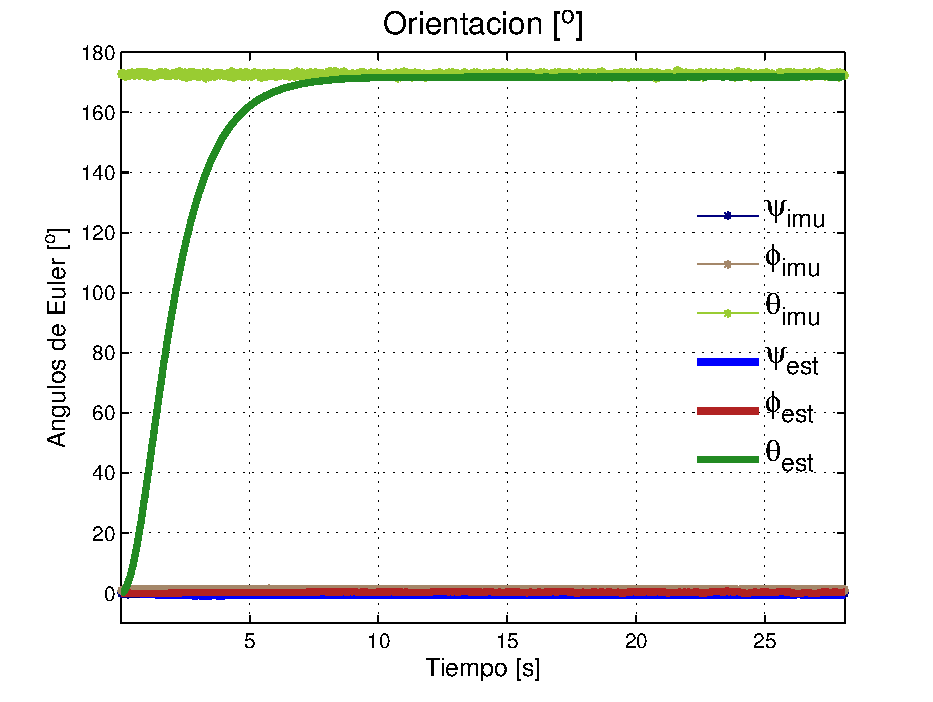
\includegraphics[width=0.47\textwidth]{./pics_kalman/euler.pdf}}
  \caption{}
  \label{fig:posyvel}
\end{figure}

En la figura \ref{fig:wq} se muestra la estimación de las velocidades angulares, junto con las medidas del giróscopo. Se puede ver claramente que la estimación del estado sigue a las medidas del giróscopo, suavizándolas y logrando robustez frente a ruidos inherentes al sensor.

Por otro lado en la figura \ref{fig:euler} se muestra tanto la orientación estimada por el filtro de Kalman, como la deducida directamente a partir de las medidas de los acelerómetros y magnetómetros de la IMU. Nuevamente se puede apreciar el buen comportamiento del filtro, suavizando notoriamente las medidas otorgadas por la imu. Además resulta intersante analizar el transitorio de la estimación del estado, es decir, el tiempo que el filtro tarda en estimar al estado. En este caso el estimador tarda aproximadamente 7 segundos en pasar de $\theta = 0$ hasta $\theta = 170$, lo cual sin duda es un tiempo totalmente inaceptable en vuelo. Este es uno de los casos más extremos ya que el ángulo $\theta$ es cercano a 180 grados. De todas maneras es un problema fácil de solucionar, se puede tomar algunas muestras de la IMU y usarlas como semilla para el filtro, y/o agregar una etapa de \emph{calentamiento} del filtro antes de que el cuadricóptero levante vuelo. A su vez, ajustando las matrices de covarianza \textbf{Q} y \textbf{R}, presentadas anteriormente, se puede lograr muy fácilmente que la estimación se acerque mucho más rápido a la medida del sensor.\\

Del resto de las variables de estado, $x$, $y$, $z$, $v_{qx}$, $v_{qy}$ y $v_{qz}$, la única que tiene realimentación, considerando una estimación de estado puramente inercial, es $z$. El resto quedan determinadas únicamente por el modelo físico, en el cual se basa la etapa de predicción del filtro de Kalman. Dicho de otro modo, la etapa de actualización/corrección del filtro no surte efecto sobre dichas variables de estado.\\

\begin{figure} [h!]
\centering
  \subfloat[Estimación de la posición]{\label{fig:pos}
    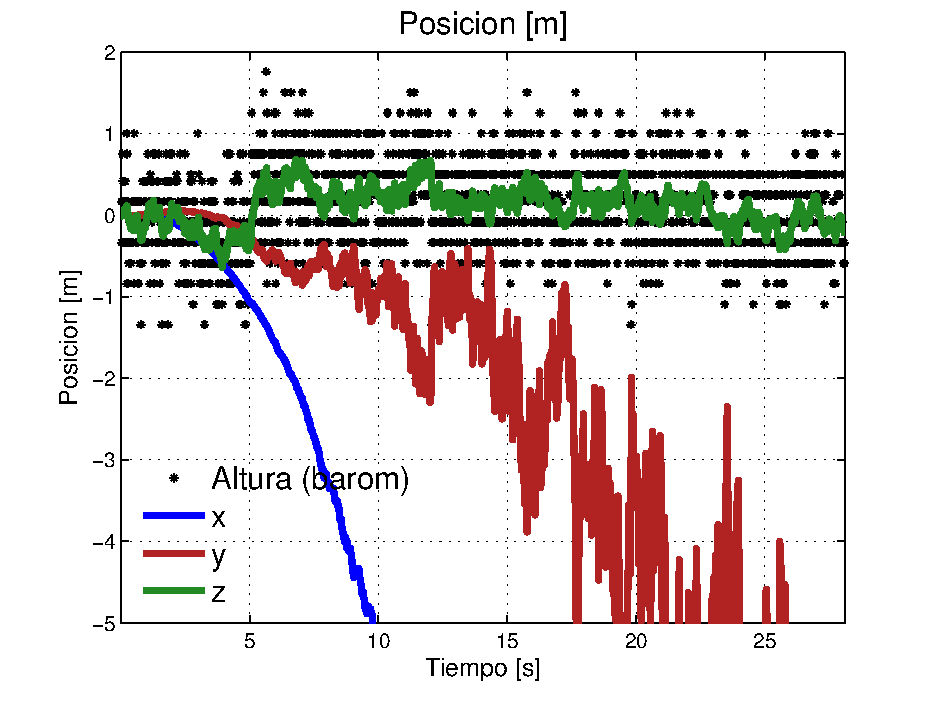
\includegraphics[width=0.47\textwidth]{./pics_kalman/pos.pdf}} \hspace{10pt}
  \subfloat[Estimación de la velocidad lineal en el sistema no inercial del cuadricóptero]{\label{fig:vq} 
    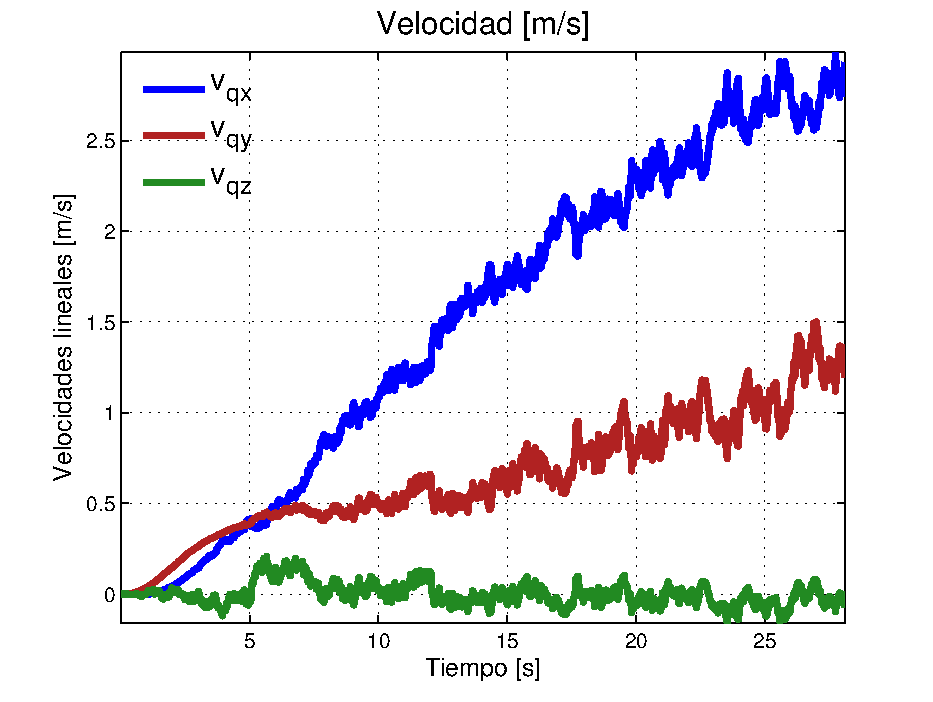
\includegraphics[width=0.47\textwidth]{./pics_kalman/vq.pdf}}
  \caption{}
  \label{fig:posyvel}
\end{figure}

Como se puede ver en la figura \ref{fig:posyvel}, la estimación de los estados que no tienen realimentación directa resulta claramente peor que el resto. De hecho, lo que ocurre por ejemplo en las velocides lineales según $x$ e $y$, es que la observación (dato obtenido del sensor) es la derivada de la variable de estado, y por ello es que se observa el carácter creciente (en valor absoluto) en la estimación del estado, causado por la integración en el tiempo del valor de aceleración otorgado por la IMU. La posición según $z$, en cambio, tiene realimentación directa del barómetro. En la figura \ref{fig:pos} se muestra en negro los datos obtenidos de dicho sensor, y sobre ellos la estimación de la altura $z$.

\subsubsection{Situación imposible}

Se simula una situación donde todos los motores se setean a una velocidad $w_{hover}$, como en el caso anterior, pero en esta oportunidad el cuadricóptero se dispone con un ángulo de $\varphi = 45^o$. Claramente es una situación de vuelo imposible ya que con esa velocidad en los motores el cuadricóptero no podría quedarse quieto en un lugar, y perdería altura. Se puede analizar la estimación de la orientación obtenida por el filtro en la figura \ref{fig:45}.

\begin{wrapfigure}{r}{0.6\textwidth}
	\begin{center}	
	\vspace{-20pt}
	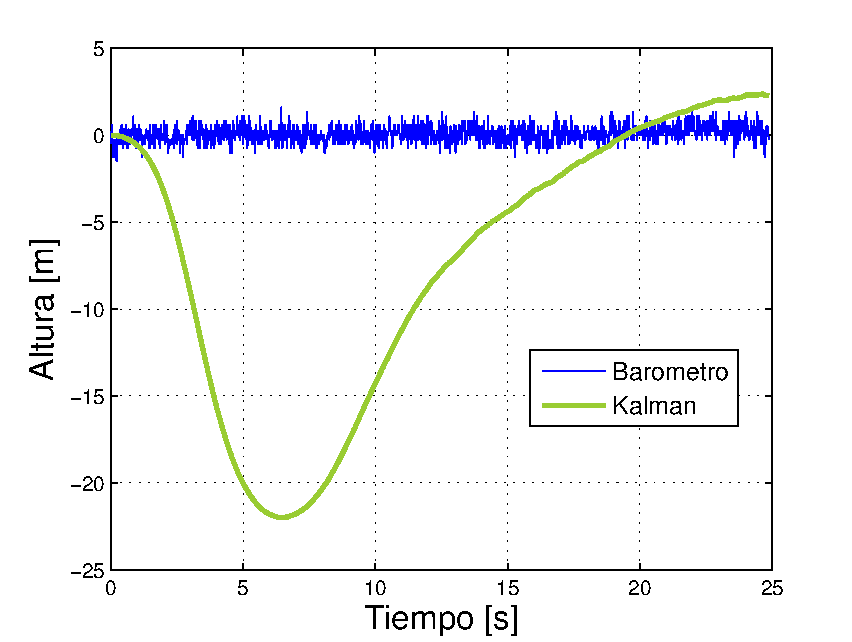
\includegraphics[width=0.45\textwidth]
		{./pics_kalman/altura_inclinado_45.pdf}
	\end{center}
	\caption{Altura - $\phi = 45^o$}
	\vspace{-20pt}
	\label{fig:45}
\end{wrapfigure}

Lo que sucede en esta situación es que la predicción de altura dice que el cuadricóptero descenderá, pero el barómetro indica altura constante. El desempeño del filtro en este caso estará determinado por la relación entre el peso que se le de a la observación y el que se le de a la predicción. En este caso el peso de la predicción es lo suficientemente grande como para que el filtro estime un estado distinto al que otorgan los sensores.

\subsection{Vuelo real}

Si bien las simulaciones resultan importantes para analizar el comportamiento del filtro en diferentes situaciones, tienen limitaciones importantes al intentar simular situaciones de vuelo reales, ya que las predicciones no serán correctas debido a la influencia de fuerzas externas no consideradas en el modelo físico (y por lo tanto, tampoco en la predicción), como estar apoyado sobre una mesa, etc. Por este motivo, es de vital importancia analizar el comportamiento del filtro sobre una situación real de vuelo.\\

%\begin{figure}[h!]
%	\centering
%	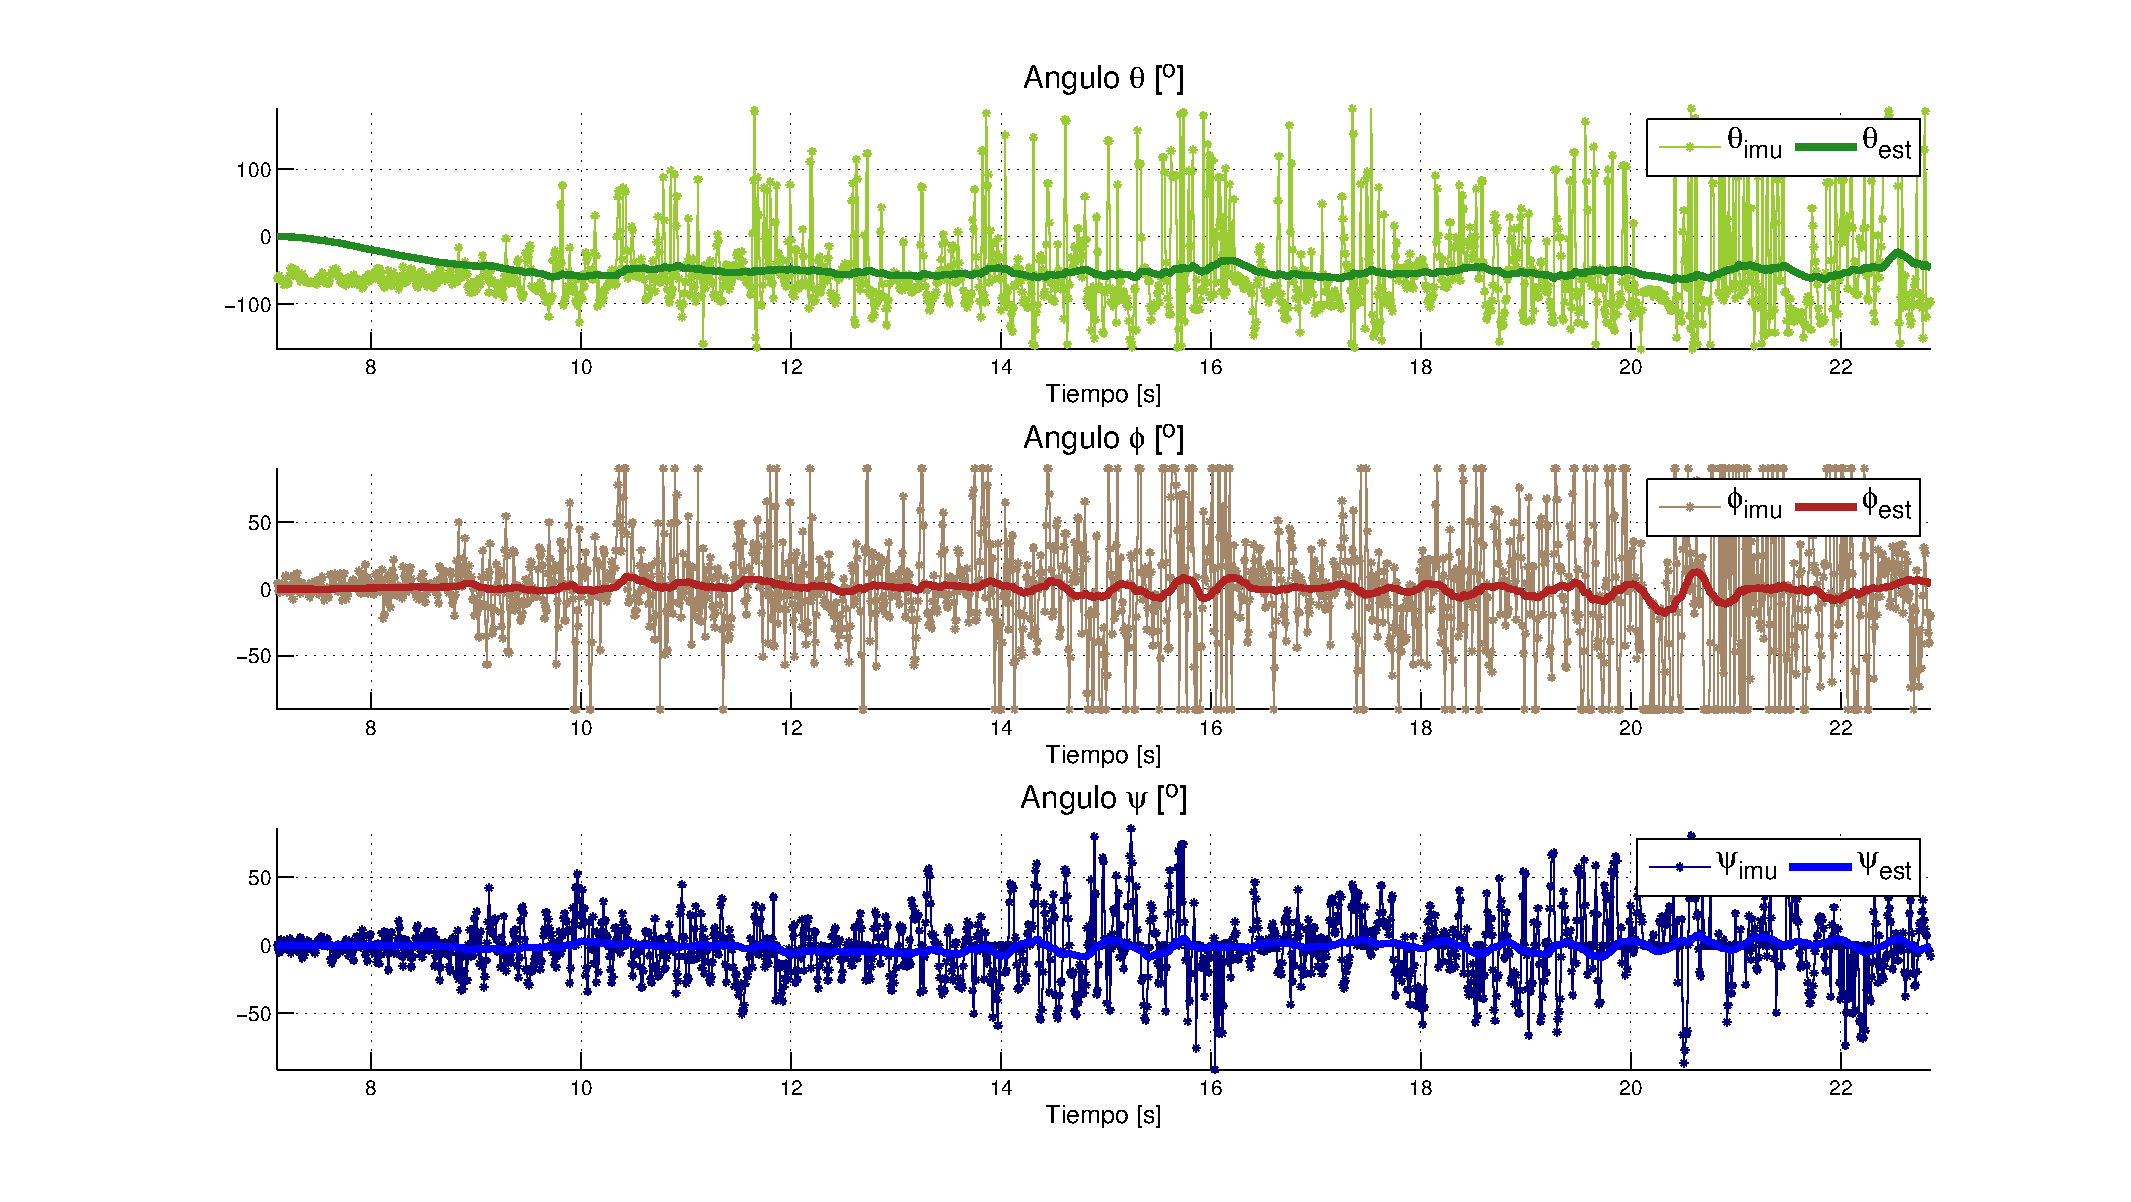
\includegraphics[width=.8\textwidth]{./pics_kalman/andando.pdf}
%	\caption{Estimación en vuelo real}
%	\label{fig:andando}
%\end{figure}
\begin{wrapfigure}{l}{0.6\textwidth}
	\vspace{-40pt}
	\begin{center}
          \hspace{-50pt}
	\vspace{-30pt}
	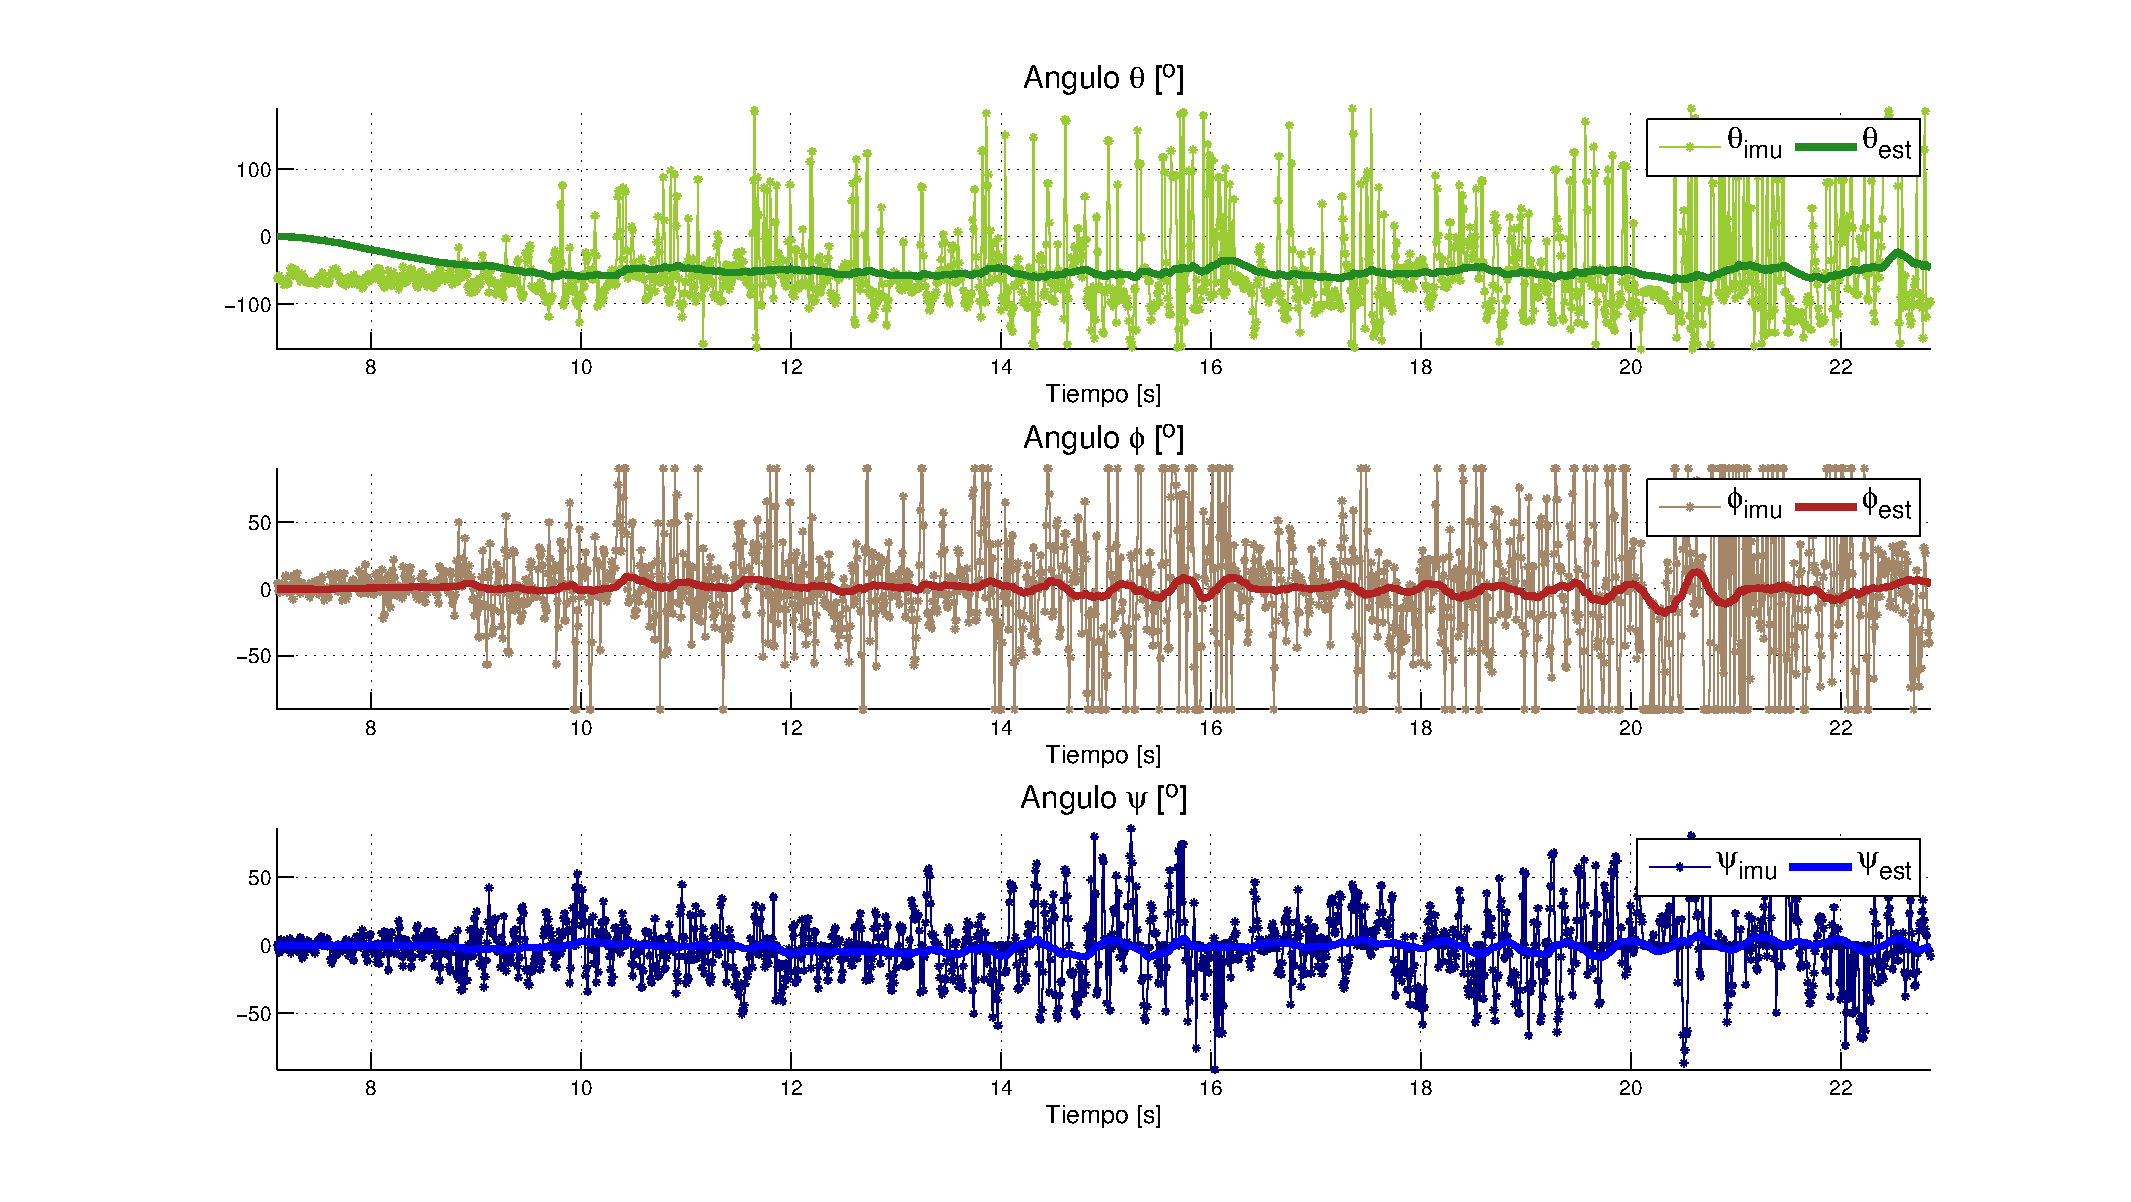
\includegraphics[width=0.65\textwidth]
		{./pics_kalman/andando.pdf}
	\end{center}
	\caption{Estimación en vuelo real}
	\label{fig:andando}
\end{wrapfigure}

En la figura \ref{fig:andando} se muestra los resultados de la estimación de la orientación del cuadricóptero. Se observa claramente un aumento del ruido de las medidas respecto a los casos simulados, llegando a picos de hasta 50 grados. De todas maneras se puede corroborar el buen funcionamiento del filtro.\\

\section{Resultados Kalman inercial + GPS}

Se realiza una simulación de trayectoria de \emph{Hovering}, introduciendo el filtro EKF que integra los datos del GPS. Éstos son simulados como si el cuadricóptero no se moviera (que es lo que efectivamente ocurre), de modo que se entrega el valor 0 a todas las posiciones

\begin{figure} [h!]
	\centering
		\subfloat[GPS - Estimación de la posición]{\label{fig:gps_pos}
			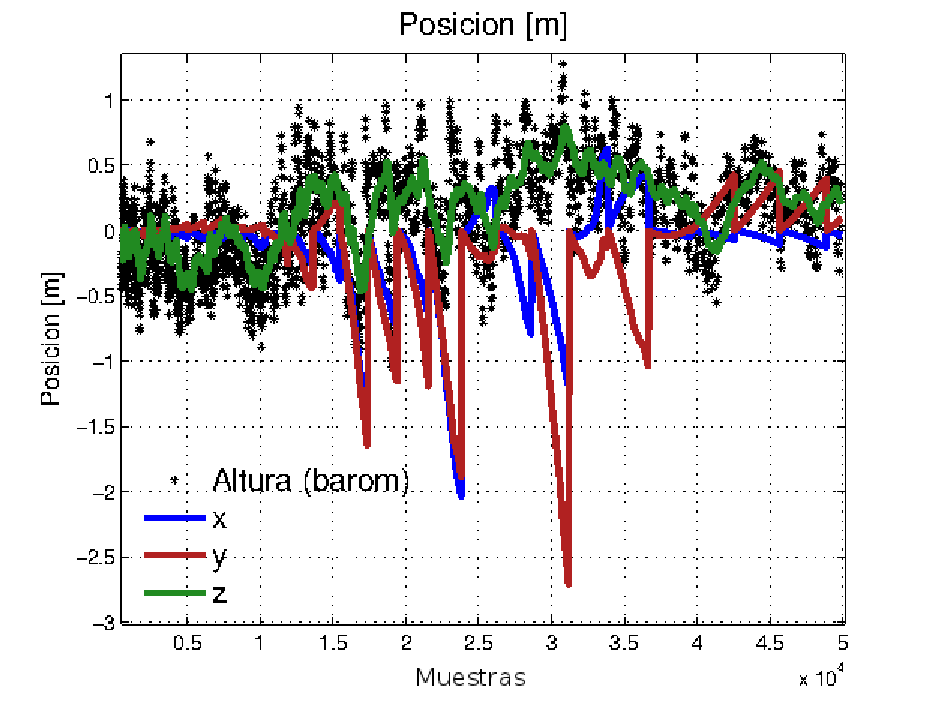
\includegraphics[width=0.47\textwidth]{./pics_kalman/gps_pos.pdf}} \hspace{10pt}
		\subfloat[GPS - Estimación de la velocidad lineal en el sistema no inercial del cuadricóptero]{\label{fig:gps_vel} 
			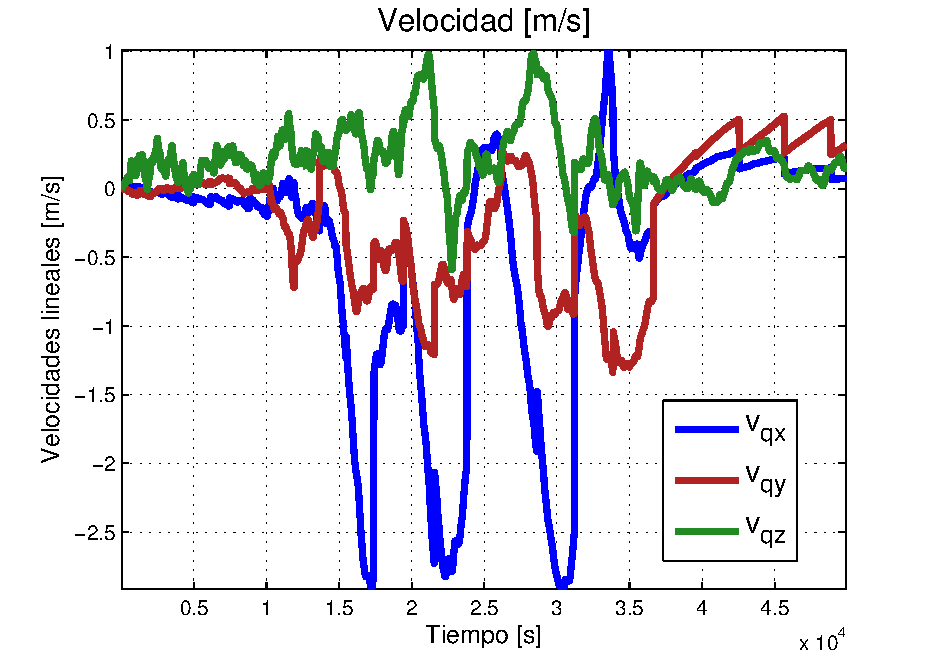
\includegraphics[width=0.47\textwidth]{./pics_kalman/gps_vel.pdf}}
		\caption{Posición y velocidad al introducir datos de GPS}
		\label{fig:gps_posyvel}
\end{figure}

Como se puede ver en la figura \ref{fig:gps_posyvel}, se actualiza la posición en ``x'' e ``y'' cada 1 segundo gracias al GPS, corrigiendo el \emph{drift} observado en la figura \ref{fig:pos}. A su vez, las velocidades lineales se acotan notoriamente gracias a la influencia de la realimentación de la posición en el filtro de Kalman.\\

Se obtienen resultados muy satisfactorios para la estimación de estados, logrando suavizar el ruido presente en los sensores, que es mayormente mecánico (y magnético en el magnetómetro), sin retrasar la señal. A su vez la información de todos los sensores es combinada para mejorar la estimación de cada una de las variables de estado, logrando resultados ampliamente mejores que lo que se lograrían utilizando la información de cada sensor por separado.

\end{document}